\documentclass[12pt]{article}
\usepackage[english]{babel}
\usepackage{fullpage, enumitem, amsmath, amssymb, graphicx, chemformula, stmaryrd, physics, booktabs, float, xfrac, mdframed, blindtext, fancyhdr, pythontex, makecell}
\usepackage[left=20mm,right=20mm,top=15mm,bottom=15mm,includeheadfoot]{geometry}

\DeclareMathSymbol{*}{\mathbin}{symbols}{"01}

\usepackage{siunitx}
\sisetup{round-mode=places, round-precision=3}

\usepackage{pgfplots}
\usepgfplotslibrary{groupplots}

\usepackage[notextcomp]{kpfonts}

\newcounter{question}[question]
\setcounter{question}{1}

\mdfdefinestyle{question}{
backgroundcolor=black!10, roundcorner=8pt, hidealllines=true, nobreak
}

\def\checkmark{\tikz\fill[scale=0.4](0,.35) -- (.25,0) -- (1,.7) -- (.25,.15) -- cycle;} 

\fancypagestyle{plain}{
\fancyhf{}%
\fancyhead[R]{}
\fancyhead[L]{}
\fancyhead[C]{}
\fancyfoot[R]{\thepage} 
\fancyfoot[C]{}
\fancyfoot[L]{Chemical Reaction Engineering}
\renewcommand{\footrulewidth}{0.4pt}
\renewcommand{\headrulewidth}{0pt}
}

\newenvironment{question}
    {\textbf{Question\;\thequestion}
    \begin{mdframed}[style=question]}
        %% Question Text %%   
    {\end{mdframed}
    \addtocounter{question}{1}} 
    
\newenvironment{solution}
    {}
        %% Solution Text %%   
    {\setcounter{equation}{0}
    \newpage} 
   
    
\title{Chemical Reaction Engineering Exam - WS2020}
\author{Fabian Hofmann -- \texttt{fabian.hofmann@jku.at}}

\setlength{\parindent}{0pt}
\definecolor{myblue}{cmyk}{1,.72,0,.38}

\makeatletter
\renewcommand{\section}{\@startsection{section}{1}{0mm}%
                                {1ex}%
                                {0.5ex}%x
                                {\color{myblue}\Large\bfseries}}
\renewcommand{\subsection}{\@startsection{subsection}{1}{0mm}%
                                {0.5ex}%
                                {0.5ex}%x
                                {\large\bfseries}}
\renewcommand{\subsubsection}{\@startsection{subsubsection}{1}{0mm}%
                                {0.5ex}%
                                {0.5ex}%x
                                {\bfseries}}
\makeatother

\begin{document}

\newcommand{\pySI}[2]{\py{'\\SI{' + str(#1) + '}{#2}'}}
\newcommand{\pyNum}[1]{\py{'\\num{' + str(#1) + '}'}}

\pagestyle{plain}
\maketitle

\begin{question}
In an indirectly cooled CSTR with a heat exchange surface of $F_W = \SI{7}{\square\meter}$, a strongly exothermic irreversible 1st order rection takes place. Initial investigations showed that the heat exchange surface must be increased by installing cooling coils inside the reactor so that the amount of heat produced can be sufficiently dissipated. The reactant is to be fed into the CSTR at a concentration of \SI{1600}{\mole\per\cubic\meter} with a volume flow of \SI{2.3}{\cubic\meter\per\hour}. The temperature of the feed mixture shall be $T_a = \SI{70}{\celsius}$. In the steady state, the operating temperature should be \SI{118}{\celsius}. The average coolant temperature $T_K$ should be \SI{95}{\celsius}. With the selected reaction conditions and operating parameters, a conversion of the reactant of \SI{98}{\percent} can be achieved. 

Further material data: Heat transfer coefficient $k_W = \SI{4. 75e5}{\joule\per\square\meter\per\hour\per\kelvin}$, reaction enthalpy $\Delta H = \SI{-195}{\kilo\joule\per\mole}$, mean density $\rho = \SI{1800}{\kilo\gram\per\cubic\meter}$ and mean specific heat capacity $c_p = \SI{2200}{\joule\per\kelvin\per\kilo\gram}$.
%
\renewcommand{\labelenumi}{\alph{enumi})}
\begin{enumerate}
\item Determine the area that must be provided for additional heat dissipation by installing cooling coils. Establish the heat balance of the statinary CSTR. What is the total area for heat exchange.
\item Give the relative cooling intensity (Stanton number) for the steady state. Also calculate the adiabatic temperature increase.
\end{enumerate}
\end{question}
%%%%%%%%%%%%%%%%%%%%%%%%%%%% Start Python calculations %%%%%%%%%%%%%%%%%%%%%%%%%%%%
\begin{pycode}
import numpy as np
import sympy as sp

# Given data
Fw = 7 #m^2
cA0 = 1600 #mol/m^3
Vdot = 2.3 #m^3/h
Ta = 70 #°C
T = 118 #°C
Tk = 95 #°C
X = 0.98 #%
kW = 4.75e5 #J/(m^2 h K)
DeltaH = -195 #kJ/mol
rho = 1809 #kg/m^3
cp = 2200 #J/(K kg)

#Calculation of the adibatic temperature increase
DeltaTad = (-1000 * DeltaH * cA0)/(rho * cp)

#Calculation of the Stanton number
St = (Ta - T + DeltaTad * X)/(T - Tk)

#Calculation of the needed heat exchange surface
FwNeed = (St * Vdot * rho * cp)/kW

#Calculation of the heat exchange surface which has to be added
FwAdd = FwNeed - Fw

\end{pycode}
%%%%%%%%%%%%%%%%%%%%%%%%%%%% End Python calculations %%%%%%%%%%%%%%%%%%%%%%%%%%%%
\begin{solution}
The heat balance of the CSTR:
%
\begin{equation}\label{eqn1:HB}
T - T_a + St*(T - T_k) = \Delta T_{ad} * X
\end{equation}
%
The adiabatic temperature increase can be calculated by:
%
\begin{equation}
\Delta T_{ad} = \frac{-\Delta H * c_{A0}}{-\nu_A * \rho * c_p} = \pySI{DeltaTad}{\kelvin} 
\end{equation}
%
By rearranging Eq. \ref{eqn1:HB} the Stanton number can be calculated
%
\begin{equation}
St = \frac{T_a - T + \Delta T_{ad} * X}{T - T_k} = \pyNum{St}
\end{equation}
%
The heat exchange surface still to be installed can be calculated according to:
%
\begin{equation}
F_{W,add} = \frac{St * \dot{V} * \rho * c_p}{k_W} - F_W = \pySI{FwAdd}{\square\meter}
\end{equation}
\end{solution}
\begin{question}
During the execution of a radical polymerization at \SI{125}{\celsius} with an initial initiator concentration of $c_{I0} = \SI{0.001}{\mol\per\liter}$, the following kinetic data were determined: The rate constant of the initiator decomposition reaction $k_z = \SI{1.09e-11}{\per\second}$, the gross rate constant $k_{Br} = \SI{3.09e-3}{\liter\tothe{1\per 2}\per\mole\tothe{1\per 2}\per\second}$
%
\renewcommand{\labelenumi}{\alph{enumi})}
\begin{enumerate}
\item Calculate the polymerisation time until a monomer conversion of \SI{70}{\percent} is reached. Write down the formulae you used for this calculation.
\end{enumerate}
\end{question}
%%%%%%%%%%%%%%%%%%%%%%%%%%%% Start Python calculations %%%%%%%%%%%%%%%%%%%%%%%%%%%%
\begin{pycode}
import numpy as np
import sympy as sp

t = sp.symbols('t', positive=True, real=True)

# Given data
T = 125 + 273.15 #K
cI0 = 0.001 #mol/L
kz = 1.09e-11 #s^-1
kBr = 3.09e-3 #L^0.5 mol^-0.5 s^-1
X = 0.7

# Calculation of the polymerization time
sol = sp.solve((2 * kBr * sp.sqrt(cI0)) / kz * (sp.exp(-kz * t / 2) - 1) - sp.log(1 - X), t)
\end{pycode}
%%%%%%%%%%%%%%%%%%%%%%%%%%%% End Python calculations %%%%%%%%%%%%%%%%%%%%%%%%%%%%
\begin{solution}
The logarithmic ratio of the monomer concentration to the initial concentration can be calculated by (CRE exercise 6):
%
\begin{equation}\label{eqn2:ratio}
\ln \left( \frac{c_M}{c_{M0}} \right) = \frac{2 * k_{Br} * \sqrt{c_{I0}}}{k_z} * \left[ \exp\left(\frac{-k_z * t}{2} \right) - 1 \right]
\end{equation}
%
The conversion in constant reaction volume is defined by:
%
\begin{equation}
X = \frac{c_{M0} - c_M}{c_{M0}} \Longrightarrow \frac{c_M}{c_{M0}} = 1 - X
\end{equation}
%
Thus Eq. \ref{eqn2:ratio} can be rearranged to:
%
\begin{align}
\begin{split}
&\ln \left( 1 - X \right) = \frac{2 * k_{Br} * \sqrt{c_{I0}}}{k_z} * \left[ \exp\left(\frac{-k_z * t}{2} \right) - 1 \right]\\
&\Longrightarrow t = -\frac{2}{k_z} * \ln \left[ \frac{\ln (1 - X) * k_z}{2 * k_{Br} * \sqrt{c_{I0}}} + 1 \right] = \pySI{sol[0]}{\second}
\end{split} 
\end{align}
\end{solution}

\begin{question}
Butyl acetat shall be produced at \SI{100}{\celsius} from acetic acid and butanol with suphuric acid as catalyst.
%%
\begin{equation*}
\ch{CH3COOH + C4H9OH -> CH3COOC4H9 + H2O}
\end{equation*}
%%
After a first approximation, it is a 2nd order reaction: \\
$r = k * c_A * c_B$ with $k = \SI{0.03}{\liter\per\mole\per\minute}$. The reaction should be terminated at a conversion of $X_A = 0.69$. The component react only in the desired form to form the butyl ester, so that the selectivity can be set to one. The production rate of the butyl ester should be \SI{109}{\kilo\gram\per\hour}. The dead time of the batch reactor for filling, heating, cooling and emptying is \SI{15}{\minute} (additional to the reaction time). The initial concentration of acetic acid is $c_{A0} = \SI{2}{\mole\per\liter}$ 
\renewcommand{\labelenumi}{\alph{enumi})}
\begin{enumerate}
 \item Calculate the Damköhler number.
 \item Calculate the residence time $\tau$.
 \item Calculate the reaction volume $V_R$ of the batch reactor.
\end{enumerate}
\end{question}
%%%%%%%%%%%%%%%%%%%%%%%%%%%% Start Python calculations %%%%%%%%%%%%%%%%%%%%%%%%%%%%
\begin{pycode}
# Given data
Mp = 116 #g mol^-1
Xa = 0.69
Sp = 1
mDot = 109 #kg h^-1
k = 0.03 #L mol^-1 min^-1
cA0 = 2 #mol/L
tD = 15 #min

# Calculation of the Damkoehler number
Da = Xa/(1-Xa)

# Calculation of the residence time
tau = Da/(k * cA0)

# Calculation of the reaction volume
Vr = 1000/60 * mDot/Mp * (tau + tD)/(cA0*Sp*Xa)
\end{pycode}
%%%%%%%%%%%%%%%%%%%%%%%%%%%% End Python calculations %%%%%%%%%%%%%%%%%%%%%%%%%%%%
\begin{solution}
The Damköhler number for a batch reactor and a reaction of 2nd order can be calculated by:
%
\begin{align}
\begin{split}
Da &= \int\limits_0^{X_A} \frac{1}{\Phi(X)}\;\mathrm{d}X = \int\limits_0^{X_A} \frac{1}{(1 - X)^2}\;\mathrm{d}X \\
&= \frac{X_A}{1 - X_A} = \pyNum{Da}
\end{split}
\end{align}
%%
The residence time can be calculated by:
%%
\begin{equation}
\tau = \frac{Da * c_{A0}}{-\nu_A * r_0} = \frac{Da}{-\nu_A * k * c_{A0}} = \pySI{tau}{\minute}
\end{equation}
%%
The selectivity towards the product can be calculated by:
%%
\begin{equation}
S_P = \frac{n_P - n_{P0}}{n_{A0} - n_A} * \frac{-\nu_A}{\nu_P} \Longrightarrow n_{A0} - n_A = \frac{n_P - n_{P0}}{S_P} * \frac{-\nu_A}{\nu_P}
\end{equation}
%%
The conversion of educt A is defined by:
%%
\begin{align}
\begin{split}
&X_A = \frac{n_{A0} - n_A}{n_{A0}} = \frac{n_P - n_{P0}}{n_{A0} * S_P} * \frac{-\nu_A}{\nu_P}\\
&\Longrightarrow n_P - n_{P0} = \frac{\nu_P}{-\nu_A} * n_{A0} * S_P * X_A
\end{split}
\end{align}
%%
The production rate is defined by:
%%
\begin{equation}\label{eqn3:dotn}
\dot{n}_P = \frac{\dot{m}_P}{M_P} = \frac{n_P - n_{P0}}{\tau + t_d} = \frac{\nu_P}{-\nu_A} * n_{A0} * S_P * X_A * \frac{1}{\tau + t_d}
\end{equation}
%%
With $n_{A0} = c_{A0} * V_R$ the reactor volume $V_R$ can be calculated by rearranging Eq. \ref{eqn3:dotn}:
%%
\begin{equation}
V_R = \frac{\dot{m}_P}{M_P} * \frac{-\nu_A}{\nu_P} * \frac{\tau + t_d}{c_{A0} * S_P * X_A} =  \pySI{Vr}{\liter}
\end{equation}
\end{solution}

\begin{question}
For a zero order reaction, the following applies: $X = Da$
%%
\renewcommand{\labelenumi}{\alph{enumi})}
\begin{enumerate}
 \item What conversion do you expect with $Da = 2$
 \item Is the Damköhler number at this reaction order depended on the temperature?
 \item How do you explain this? Use equations for the explanation!
\end{enumerate}
\end{question}
%%%%%%%%%%%%%%%%%%%%%%%%%%%% Start Python calculations %%%%%%%%%%%%%%%%%%%%%%%%%%%%
\begin{pycode}

\end{pycode}
%%%%%%%%%%%%%%%%%%%%%%%%%%%% End Python calculations %%%%%%%%%%%%%%%%%%%%%%%%%%%%
\begin{solution}
The conversion can only be \SI{100}{\percent} even if $Da = 2$. The higher Damköhler number can be attributed to the temperature.
%%
\begin{equation}
Da = \frac{-\nu_A * r_0 * \tau}{c_{A0}}
\end{equation}
The reaction rate $r_0$ at the begin of the reaction $(X = 0)$:
%%
\begin{equation}
r_0 = k(T) = k_{\infty} * \exp\left(\frac{-E_A}{R * T}\right)
\end{equation}
\end{solution}

\begin{question}
For an exothermic reaction, draw the expected course of reaction of the educt A $(c_A)$ as a functiuon of time $(t)$ and location $(x)$ espacially for the measurement location $z_0$ and $z_1$. The reaction proceeds according to the scheme
%%
\begin{equation*}
\ch{A -> P}
\end{equation*}
No cooling and the reactors behave ideal.
\end{question}
\begin{solution}
Time and location dependence on concentration:
\begin{center}
% This file was created by tikzplotlib v0.9.8.
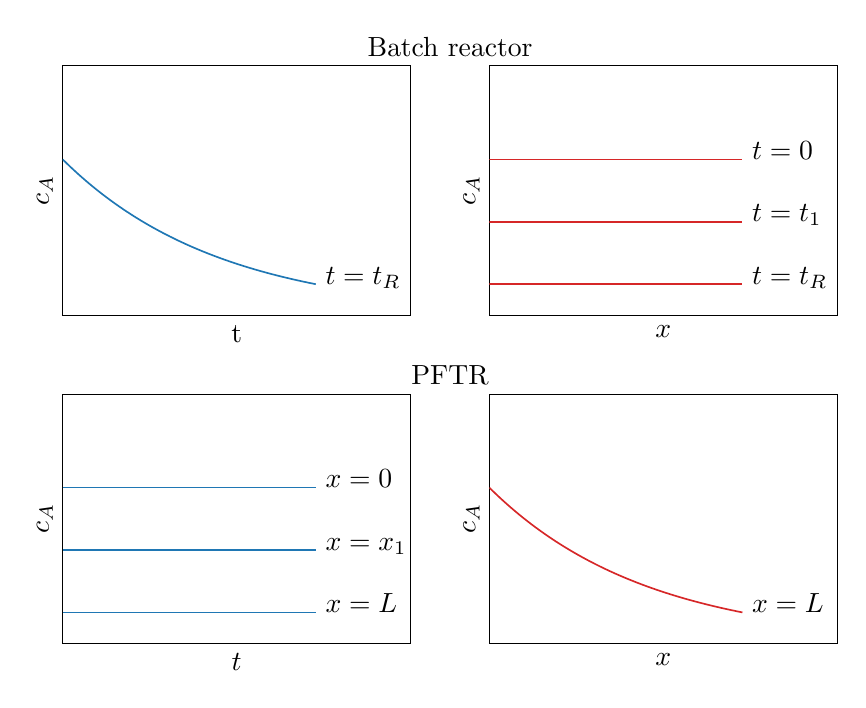
\begin{tikzpicture}

\definecolor{color0}{rgb}{0.12156862745098,0.466666666666667,0.705882352941177}
\definecolor{color1}{rgb}{0.83921568627451,0.152941176470588,0.156862745098039}

\begin{groupplot}[group style={
                group name=my plots,
                group size=2 by 2,
                vertical sep=1cm
            }]
\nextgroupplot[
height=4.75cm,
ylabel near ticks,
xlabel near ticks,
xtick=\empty,
ytick=\empty,
width=6cm,
xlabel={t},
xmin=0, xmax=2.75,
ylabel={\(\displaystyle c_A\)},
ymin=0, ymax=8
]
\addplot [semithick, color0]
table {%
0 5
0.0202020202020202 4.91937241196215
0.0404040404040404 4.84004498551486
0.0606060606060606 4.7619967548795
0.0808080808080808 4.6852070923615
0.101010101010101 4.60965570289851
0.121212121212121 4.53532261869659
0.141414141414141 4.46218819395278
0.161616161616162 4.3902330996629
0.181818181818182 4.31943831851295
0.202020202020202 4.24978513985296
0.222222222222222 4.18125515475187
0.242424242424242 4.11383025113217
0.262626262626263 4.04749260898298
0.282828282828283 3.98222469565032
0.303030303030303 3.91800926120331
0.323232323232323 3.85482933387515
0.343434343434343 3.79266821557757
0.363636363636364 3.7315094774876
0.383838383838384 3.67133695570556
0.404040404040404 3.612134746983
0.424242424242424 3.55388720451961
0.444444444444444 3.49657893382781
0.464646464646465 3.44019478866411
0.484848484848485 3.38471986702604
0.505050505050505 3.33013950721362
0.525252525252525 3.27643928395438
0.545454545454546 3.22360500459084
0.565656565656566 3.17162270532945
0.585858585858586 3.12047864755009
0.606060606060606 3.07015931417498
0.626262626262626 3.0206514060962
0.646464646464647 2.97194183866087
0.666666666666667 2.92401773821287
0.686868686868687 2.87686643869047
0.707070707070707 2.83047547827874
0.727272727272727 2.78483259611596
0.747474747474748 2.73992572905315
0.767676767676768 2.69574300846587
0.787878787878788 2.65227275711737
0.808080808080808 2.60950348607239
0.828282828282828 2.56742389166072
0.848484848484849 2.52602285248965
0.868686868686869 2.4852894265047
0.888888888888889 2.44521284809769
0.909090909090909 2.40578252526143
0.929292929292929 2.36698803679034
0.94949494949495 2.32881912952617
0.96969696969697 2.29126571564815
0.98989898989899 2.25431787000685
1.01010101010101 2.21796582750099
1.03030303030303 2.18219998049663
1.05050505050505 2.14701087628789
1.07070707070707 2.11238921459867
1.09090909090909 2.07832584512462
1.11111111111111 2.04481176511479
1.13131313131313 2.01183811699227
1.15151515151515 1.97939618601313
1.17171717171717 1.94747739796321
1.19191919191919 1.91607331689201
1.21212121212121 1.88517564288307
1.23232323232323 1.8547762098604
1.25252525252525 1.82486698343019
1.27272727272727 1.79544005875742
1.29292929292929 1.76648765847659
1.31313131313131 1.73800213063627
1.33333333333333 1.7099759466767
1.35353535353535 1.68240169944004
1.37373737373737 1.65527210121271
1.39393939393939 1.62857998179929
1.41414141414141 1.60231828662745
1.43434343434343 1.5764800748835
1.45454545454545 1.55105851767799
1.47474747474747 1.5260468962408
1.4949494949495 1.50143860014549
1.51515151515152 1.47722712556216
1.53535353535354 1.45340607353852
1.55555555555556 1.42996914830873
1.57575757575758 1.40691015562939
1.5959595959596 1.38422300114252
1.61616161616162 1.36190168876479
1.63636363636364 1.33994031910284
1.65656565656566 1.31833308789405
1.67676767676768 1.29707428447257
1.6969696969697 1.27615829025999
1.71717171717172 1.25557957728035
1.73737373737374 1.23533270669921
1.75757575757576 1.21541232738612
1.77777777777778 1.1958131745004
1.7979797979798 1.17653006809963
1.81818181818182 1.15755791177065
1.83838383838384 1.13889169128261
1.85858585858586 1.12052647326172
1.87878787878788 1.10245740388739
1.8989898989899 1.08467970760941
1.91919191919192 1.06718868588578
1.93939393939394 1.04997971594093
1.95959595959596 1.03304824954393
1.97979797979798 1.01638981180644
2 1
};
\draw (axis cs:2,1) node[
  anchor=base west,
  text=black,
  rotate=0.0
]{$t = t_R$};

\nextgroupplot[
height=4.75cm,
ylabel near ticks,
xlabel near ticks,
xtick=\empty,
ytick=\empty,
width=6cm,
xlabel={\(\displaystyle x\)},
xmin=0, xmax=2.75,
ylabel={\(\displaystyle c_A\)},
ymin=0, ymax=8
]
\addplot [semithick, color1]
table {%
0 5
0.0202020202020202 5
0.0404040404040404 5
0.0606060606060606 5
0.0808080808080808 5
0.101010101010101 5
0.121212121212121 5
0.141414141414141 5
0.161616161616162 5
0.181818181818182 5
0.202020202020202 5
0.222222222222222 5
0.242424242424242 5
0.262626262626263 5
0.282828282828283 5
0.303030303030303 5
0.323232323232323 5
0.343434343434343 5
0.363636363636364 5
0.383838383838384 5
0.404040404040404 5
0.424242424242424 5
0.444444444444444 5
0.464646464646465 5
0.484848484848485 5
0.505050505050505 5
0.525252525252525 5
0.545454545454546 5
0.565656565656566 5
0.585858585858586 5
0.606060606060606 5
0.626262626262626 5
0.646464646464647 5
0.666666666666667 5
0.686868686868687 5
0.707070707070707 5
0.727272727272727 5
0.747474747474748 5
0.767676767676768 5
0.787878787878788 5
0.808080808080808 5
0.828282828282828 5
0.848484848484849 5
0.868686868686869 5
0.888888888888889 5
0.909090909090909 5
0.929292929292929 5
0.94949494949495 5
0.96969696969697 5
0.98989898989899 5
1.01010101010101 5
1.03030303030303 5
1.05050505050505 5
1.07070707070707 5
1.09090909090909 5
1.11111111111111 5
1.13131313131313 5
1.15151515151515 5
1.17171717171717 5
1.19191919191919 5
1.21212121212121 5
1.23232323232323 5
1.25252525252525 5
1.27272727272727 5
1.29292929292929 5
1.31313131313131 5
1.33333333333333 5
1.35353535353535 5
1.37373737373737 5
1.39393939393939 5
1.41414141414141 5
1.43434343434343 5
1.45454545454545 5
1.47474747474747 5
1.4949494949495 5
1.51515151515152 5
1.53535353535354 5
1.55555555555556 5
1.57575757575758 5
1.5959595959596 5
1.61616161616162 5
1.63636363636364 5
1.65656565656566 5
1.67676767676768 5
1.6969696969697 5
1.71717171717172 5
1.73737373737374 5
1.75757575757576 5
1.77777777777778 5
1.7979797979798 5
1.81818181818182 5
1.83838383838384 5
1.85858585858586 5
1.87878787878788 5
1.8989898989899 5
1.91919191919192 5
1.93939393939394 5
1.95959595959596 5
1.97979797979798 5
2 5
};
\addplot [semithick, color1]
table {%
0 3
0.0202020202020202 3
0.0404040404040404 3
0.0606060606060606 3
0.0808080808080808 3
0.101010101010101 3
0.121212121212121 3
0.141414141414141 3
0.161616161616162 3
0.181818181818182 3
0.202020202020202 3
0.222222222222222 3
0.242424242424242 3
0.262626262626263 3
0.282828282828283 3
0.303030303030303 3
0.323232323232323 3
0.343434343434343 3
0.363636363636364 3
0.383838383838384 3
0.404040404040404 3
0.424242424242424 3
0.444444444444444 3
0.464646464646465 3
0.484848484848485 3
0.505050505050505 3
0.525252525252525 3
0.545454545454546 3
0.565656565656566 3
0.585858585858586 3
0.606060606060606 3
0.626262626262626 3
0.646464646464647 3
0.666666666666667 3
0.686868686868687 3
0.707070707070707 3
0.727272727272727 3
0.747474747474748 3
0.767676767676768 3
0.787878787878788 3
0.808080808080808 3
0.828282828282828 3
0.848484848484849 3
0.868686868686869 3
0.888888888888889 3
0.909090909090909 3
0.929292929292929 3
0.94949494949495 3
0.96969696969697 3
0.98989898989899 3
1.01010101010101 3
1.03030303030303 3
1.05050505050505 3
1.07070707070707 3
1.09090909090909 3
1.11111111111111 3
1.13131313131313 3
1.15151515151515 3
1.17171717171717 3
1.19191919191919 3
1.21212121212121 3
1.23232323232323 3
1.25252525252525 3
1.27272727272727 3
1.29292929292929 3
1.31313131313131 3
1.33333333333333 3
1.35353535353535 3
1.37373737373737 3
1.39393939393939 3
1.41414141414141 3
1.43434343434343 3
1.45454545454545 3
1.47474747474747 3
1.4949494949495 3
1.51515151515152 3
1.53535353535354 3
1.55555555555556 3
1.57575757575758 3
1.5959595959596 3
1.61616161616162 3
1.63636363636364 3
1.65656565656566 3
1.67676767676768 3
1.6969696969697 3
1.71717171717172 3
1.73737373737374 3
1.75757575757576 3
1.77777777777778 3
1.7979797979798 3
1.81818181818182 3
1.83838383838384 3
1.85858585858586 3
1.87878787878788 3
1.8989898989899 3
1.91919191919192 3
1.93939393939394 3
1.95959595959596 3
1.97979797979798 3
2 3
};
\addplot [semithick, color1]
table {%
0 1
0.0202020202020202 1
0.0404040404040404 1
0.0606060606060606 1
0.0808080808080808 1
0.101010101010101 1
0.121212121212121 1
0.141414141414141 1
0.161616161616162 1
0.181818181818182 1
0.202020202020202 1
0.222222222222222 1
0.242424242424242 1
0.262626262626263 1
0.282828282828283 1
0.303030303030303 1
0.323232323232323 1
0.343434343434343 1
0.363636363636364 1
0.383838383838384 1
0.404040404040404 1
0.424242424242424 1
0.444444444444444 1
0.464646464646465 1
0.484848484848485 1
0.505050505050505 1
0.525252525252525 1
0.545454545454546 1
0.565656565656566 1
0.585858585858586 1
0.606060606060606 1
0.626262626262626 1
0.646464646464647 1
0.666666666666667 1
0.686868686868687 1
0.707070707070707 1
0.727272727272727 1
0.747474747474748 1
0.767676767676768 1
0.787878787878788 1
0.808080808080808 1
0.828282828282828 1
0.848484848484849 1
0.868686868686869 1
0.888888888888889 1
0.909090909090909 1
0.929292929292929 1
0.94949494949495 1
0.96969696969697 1
0.98989898989899 1
1.01010101010101 1
1.03030303030303 1
1.05050505050505 1
1.07070707070707 1
1.09090909090909 1
1.11111111111111 1
1.13131313131313 1
1.15151515151515 1
1.17171717171717 1
1.19191919191919 1
1.21212121212121 1
1.23232323232323 1
1.25252525252525 1
1.27272727272727 1
1.29292929292929 1
1.31313131313131 1
1.33333333333333 1
1.35353535353535 1
1.37373737373737 1
1.39393939393939 1
1.41414141414141 1
1.43434343434343 1
1.45454545454545 1
1.47474747474747 1
1.4949494949495 1
1.51515151515152 1
1.53535353535354 1
1.55555555555556 1
1.57575757575758 1
1.5959595959596 1
1.61616161616162 1
1.63636363636364 1
1.65656565656566 1
1.67676767676768 1
1.6969696969697 1
1.71717171717172 1
1.73737373737374 1
1.75757575757576 1
1.77777777777778 1
1.7979797979798 1
1.81818181818182 1
1.83838383838384 1
1.85858585858586 1
1.87878787878788 1
1.8989898989899 1
1.91919191919192 1
1.93939393939394 1
1.95959595959596 1
1.97979797979798 1
2 1
};
\draw (axis cs:2,5) node[
  anchor=base west,
  text=black,
  rotate=0.0
]{$t = 0$};
\draw (axis cs:2,3) node[
  anchor=base west,
  text=black,
  rotate=0.0
]{$t = t_1$};
\draw (axis cs:2,1) node[
  anchor=base west,
  text=black,
  rotate=0.0
]{$t = t_R$};

\nextgroupplot[
height=4.75cm,
ylabel near ticks,
xlabel near ticks,
xtick=\empty,
ytick=\empty,
width=6cm,
xlabel={\(\displaystyle t\)},
xmin=0, xmax=2.75,
ylabel={\(\displaystyle c_A\)},
ymin=0, ymax=8
]
\addplot [semithick, color0]
table {%
0 5
0.0202020202020202 5
0.0404040404040404 5
0.0606060606060606 5
0.0808080808080808 5
0.101010101010101 5
0.121212121212121 5
0.141414141414141 5
0.161616161616162 5
0.181818181818182 5
0.202020202020202 5
0.222222222222222 5
0.242424242424242 5
0.262626262626263 5
0.282828282828283 5
0.303030303030303 5
0.323232323232323 5
0.343434343434343 5
0.363636363636364 5
0.383838383838384 5
0.404040404040404 5
0.424242424242424 5
0.444444444444444 5
0.464646464646465 5
0.484848484848485 5
0.505050505050505 5
0.525252525252525 5
0.545454545454546 5
0.565656565656566 5
0.585858585858586 5
0.606060606060606 5
0.626262626262626 5
0.646464646464647 5
0.666666666666667 5
0.686868686868687 5
0.707070707070707 5
0.727272727272727 5
0.747474747474748 5
0.767676767676768 5
0.787878787878788 5
0.808080808080808 5
0.828282828282828 5
0.848484848484849 5
0.868686868686869 5
0.888888888888889 5
0.909090909090909 5
0.929292929292929 5
0.94949494949495 5
0.96969696969697 5
0.98989898989899 5
1.01010101010101 5
1.03030303030303 5
1.05050505050505 5
1.07070707070707 5
1.09090909090909 5
1.11111111111111 5
1.13131313131313 5
1.15151515151515 5
1.17171717171717 5
1.19191919191919 5
1.21212121212121 5
1.23232323232323 5
1.25252525252525 5
1.27272727272727 5
1.29292929292929 5
1.31313131313131 5
1.33333333333333 5
1.35353535353535 5
1.37373737373737 5
1.39393939393939 5
1.41414141414141 5
1.43434343434343 5
1.45454545454545 5
1.47474747474747 5
1.4949494949495 5
1.51515151515152 5
1.53535353535354 5
1.55555555555556 5
1.57575757575758 5
1.5959595959596 5
1.61616161616162 5
1.63636363636364 5
1.65656565656566 5
1.67676767676768 5
1.6969696969697 5
1.71717171717172 5
1.73737373737374 5
1.75757575757576 5
1.77777777777778 5
1.7979797979798 5
1.81818181818182 5
1.83838383838384 5
1.85858585858586 5
1.87878787878788 5
1.8989898989899 5
1.91919191919192 5
1.93939393939394 5
1.95959595959596 5
1.97979797979798 5
2 5
};
\addplot [semithick, color0]
table {%
0 3
0.0202020202020202 3
0.0404040404040404 3
0.0606060606060606 3
0.0808080808080808 3
0.101010101010101 3
0.121212121212121 3
0.141414141414141 3
0.161616161616162 3
0.181818181818182 3
0.202020202020202 3
0.222222222222222 3
0.242424242424242 3
0.262626262626263 3
0.282828282828283 3
0.303030303030303 3
0.323232323232323 3
0.343434343434343 3
0.363636363636364 3
0.383838383838384 3
0.404040404040404 3
0.424242424242424 3
0.444444444444444 3
0.464646464646465 3
0.484848484848485 3
0.505050505050505 3
0.525252525252525 3
0.545454545454546 3
0.565656565656566 3
0.585858585858586 3
0.606060606060606 3
0.626262626262626 3
0.646464646464647 3
0.666666666666667 3
0.686868686868687 3
0.707070707070707 3
0.727272727272727 3
0.747474747474748 3
0.767676767676768 3
0.787878787878788 3
0.808080808080808 3
0.828282828282828 3
0.848484848484849 3
0.868686868686869 3
0.888888888888889 3
0.909090909090909 3
0.929292929292929 3
0.94949494949495 3
0.96969696969697 3
0.98989898989899 3
1.01010101010101 3
1.03030303030303 3
1.05050505050505 3
1.07070707070707 3
1.09090909090909 3
1.11111111111111 3
1.13131313131313 3
1.15151515151515 3
1.17171717171717 3
1.19191919191919 3
1.21212121212121 3
1.23232323232323 3
1.25252525252525 3
1.27272727272727 3
1.29292929292929 3
1.31313131313131 3
1.33333333333333 3
1.35353535353535 3
1.37373737373737 3
1.39393939393939 3
1.41414141414141 3
1.43434343434343 3
1.45454545454545 3
1.47474747474747 3
1.4949494949495 3
1.51515151515152 3
1.53535353535354 3
1.55555555555556 3
1.57575757575758 3
1.5959595959596 3
1.61616161616162 3
1.63636363636364 3
1.65656565656566 3
1.67676767676768 3
1.6969696969697 3
1.71717171717172 3
1.73737373737374 3
1.75757575757576 3
1.77777777777778 3
1.7979797979798 3
1.81818181818182 3
1.83838383838384 3
1.85858585858586 3
1.87878787878788 3
1.8989898989899 3
1.91919191919192 3
1.93939393939394 3
1.95959595959596 3
1.97979797979798 3
2 3
};
\addplot [semithick, color0]
table {%
0 1
0.0202020202020202 1
0.0404040404040404 1
0.0606060606060606 1
0.0808080808080808 1
0.101010101010101 1
0.121212121212121 1
0.141414141414141 1
0.161616161616162 1
0.181818181818182 1
0.202020202020202 1
0.222222222222222 1
0.242424242424242 1
0.262626262626263 1
0.282828282828283 1
0.303030303030303 1
0.323232323232323 1
0.343434343434343 1
0.363636363636364 1
0.383838383838384 1
0.404040404040404 1
0.424242424242424 1
0.444444444444444 1
0.464646464646465 1
0.484848484848485 1
0.505050505050505 1
0.525252525252525 1
0.545454545454546 1
0.565656565656566 1
0.585858585858586 1
0.606060606060606 1
0.626262626262626 1
0.646464646464647 1
0.666666666666667 1
0.686868686868687 1
0.707070707070707 1
0.727272727272727 1
0.747474747474748 1
0.767676767676768 1
0.787878787878788 1
0.808080808080808 1
0.828282828282828 1
0.848484848484849 1
0.868686868686869 1
0.888888888888889 1
0.909090909090909 1
0.929292929292929 1
0.94949494949495 1
0.96969696969697 1
0.98989898989899 1
1.01010101010101 1
1.03030303030303 1
1.05050505050505 1
1.07070707070707 1
1.09090909090909 1
1.11111111111111 1
1.13131313131313 1
1.15151515151515 1
1.17171717171717 1
1.19191919191919 1
1.21212121212121 1
1.23232323232323 1
1.25252525252525 1
1.27272727272727 1
1.29292929292929 1
1.31313131313131 1
1.33333333333333 1
1.35353535353535 1
1.37373737373737 1
1.39393939393939 1
1.41414141414141 1
1.43434343434343 1
1.45454545454545 1
1.47474747474747 1
1.4949494949495 1
1.51515151515152 1
1.53535353535354 1
1.55555555555556 1
1.57575757575758 1
1.5959595959596 1
1.61616161616162 1
1.63636363636364 1
1.65656565656566 1
1.67676767676768 1
1.6969696969697 1
1.71717171717172 1
1.73737373737374 1
1.75757575757576 1
1.77777777777778 1
1.7979797979798 1
1.81818181818182 1
1.83838383838384 1
1.85858585858586 1
1.87878787878788 1
1.8989898989899 1
1.91919191919192 1
1.93939393939394 1
1.95959595959596 1
1.97979797979798 1
2 1
};
\draw (axis cs:2,5) node[
  anchor=base west,
  text=black,
  rotate=0.0
]{$x = 0$};
\draw (axis cs:2,3) node[
  anchor=base west,
  text=black,
  rotate=0.0
]{$x = x_1$};
\draw (axis cs:2,1) node[
  anchor=base west,
  text=black,
  rotate=0.0
]{$x = L$};

\nextgroupplot[
height=4.75cm,
ylabel near ticks,
xlabel near ticks,
xtick=\empty,
ytick=\empty,
width=6cm,
xlabel={\(\displaystyle x\)},
xmin=0, xmax=2.75,
ylabel={\(\displaystyle c_A\)},
ymin=0, ymax=8
]
\addplot [semithick, color1]
table {%
0 5
0.0202020202020202 4.91937241196215
0.0404040404040404 4.84004498551486
0.0606060606060606 4.7619967548795
0.0808080808080808 4.6852070923615
0.101010101010101 4.60965570289851
0.121212121212121 4.53532261869659
0.141414141414141 4.46218819395278
0.161616161616162 4.3902330996629
0.181818181818182 4.31943831851295
0.202020202020202 4.24978513985296
0.222222222222222 4.18125515475187
0.242424242424242 4.11383025113217
0.262626262626263 4.04749260898298
0.282828282828283 3.98222469565032
0.303030303030303 3.91800926120331
0.323232323232323 3.85482933387515
0.343434343434343 3.79266821557757
0.363636363636364 3.7315094774876
0.383838383838384 3.67133695570556
0.404040404040404 3.612134746983
0.424242424242424 3.55388720451961
0.444444444444444 3.49657893382781
0.464646464646465 3.44019478866411
0.484848484848485 3.38471986702604
0.505050505050505 3.33013950721362
0.525252525252525 3.27643928395438
0.545454545454546 3.22360500459084
0.565656565656566 3.17162270532945
0.585858585858586 3.12047864755009
0.606060606060606 3.07015931417498
0.626262626262626 3.0206514060962
0.646464646464647 2.97194183866087
0.666666666666667 2.92401773821287
0.686868686868687 2.87686643869047
0.707070707070707 2.83047547827874
0.727272727272727 2.78483259611596
0.747474747474748 2.73992572905315
0.767676767676768 2.69574300846587
0.787878787878788 2.65227275711737
0.808080808080808 2.60950348607239
0.828282828282828 2.56742389166072
0.848484848484849 2.52602285248965
0.868686868686869 2.4852894265047
0.888888888888889 2.44521284809769
0.909090909090909 2.40578252526143
0.929292929292929 2.36698803679034
0.94949494949495 2.32881912952617
0.96969696969697 2.29126571564815
0.98989898989899 2.25431787000685
1.01010101010101 2.21796582750099
1.03030303030303 2.18219998049663
1.05050505050505 2.14701087628789
1.07070707070707 2.11238921459867
1.09090909090909 2.07832584512462
1.11111111111111 2.04481176511479
1.13131313131313 2.01183811699227
1.15151515151515 1.97939618601313
1.17171717171717 1.94747739796321
1.19191919191919 1.91607331689201
1.21212121212121 1.88517564288307
1.23232323232323 1.8547762098604
1.25252525252525 1.82486698343019
1.27272727272727 1.79544005875742
1.29292929292929 1.76648765847659
1.31313131313131 1.73800213063627
1.33333333333333 1.7099759466767
1.35353535353535 1.68240169944004
1.37373737373737 1.65527210121271
1.39393939393939 1.62857998179929
1.41414141414141 1.60231828662745
1.43434343434343 1.5764800748835
1.45454545454545 1.55105851767799
1.47474747474747 1.5260468962408
1.4949494949495 1.50143860014549
1.51515151515152 1.47722712556216
1.53535353535354 1.45340607353852
1.55555555555556 1.42996914830873
1.57575757575758 1.40691015562939
1.5959595959596 1.38422300114252
1.61616161616162 1.36190168876479
1.63636363636364 1.33994031910284
1.65656565656566 1.31833308789405
1.67676767676768 1.29707428447257
1.6969696969697 1.27615829025999
1.71717171717172 1.25557957728035
1.73737373737374 1.23533270669921
1.75757575757576 1.21541232738612
1.77777777777778 1.1958131745004
1.7979797979798 1.17653006809963
1.81818181818182 1.15755791177065
1.83838383838384 1.13889169128261
1.85858585858586 1.12052647326172
1.87878787878788 1.10245740388739
1.8989898989899 1.08467970760941
1.91919191919192 1.06718868588578
1.93939393939394 1.04997971594093
1.95959595959596 1.03304824954393
1.97979797979798 1.01638981180644
2 1
};
\draw (axis cs:2,1) node[
  anchor=base west,
  text=black,
  rotate=0.0
]{$x = L$};
\end{groupplot}
\node[anchor=south] at ($(my plots c1r1.north east)!0.5!(my plots c2r1.north west)$){Batch reactor};
\node[anchor=south] at ($(my plots c1r2.north east)!0.5!(my plots c2r2.north west)$){PFTR};
\end{tikzpicture}

\end{center}
Time and location dependence on temperature:
\begin{center}
% This file was created by tikzplotlib v0.9.8.
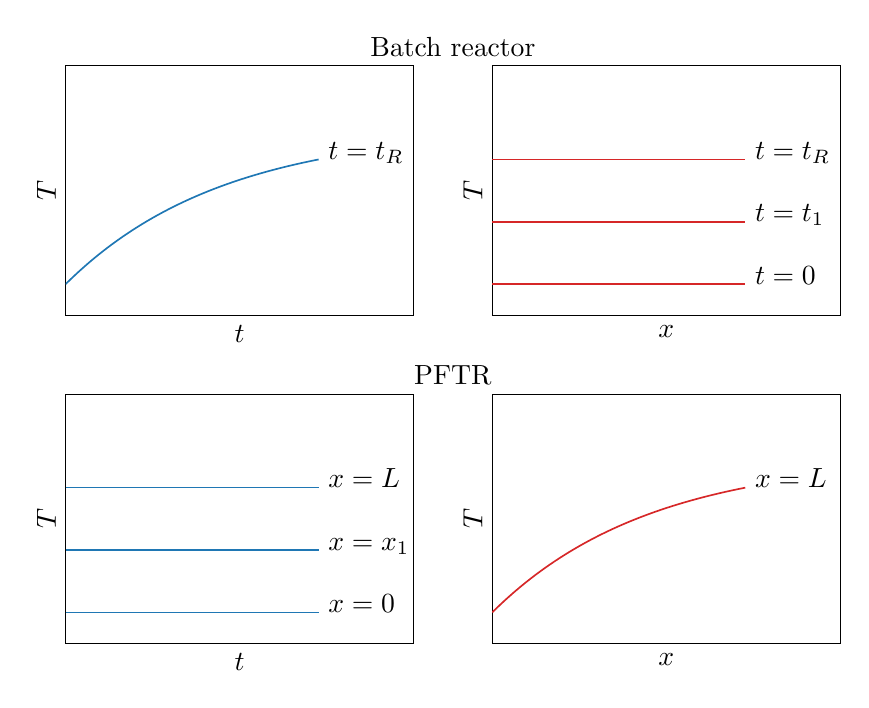
\begin{tikzpicture}

\definecolor{color0}{rgb}{0.12156862745098,0.466666666666667,0.705882352941177}
\definecolor{color1}{rgb}{0.83921568627451,0.152941176470588,0.156862745098039}

\begin{groupplot}[group style={
                group name=my plots,
                group size=2 by 2,
                vertical sep=1cm
            }]
\nextgroupplot[
height=4.75cm,
ylabel near ticks,
xlabel near ticks,
xtick=\empty,
ytick=\empty,
width=6cm,
xlabel={\(\displaystyle t\)},
xmin=0, xmax=2.75,
ylabel={\(\displaystyle T\)},
ymin=0, ymax=8
]
\addplot [semithick, color0]
table {%
0 1
0.0202020202020202 1.08062758803785
0.0404040404040404 1.15995501448514
0.0606060606060606 1.2380032451205
0.0808080808080808 1.3147929076385
0.101010101010101 1.39034429710149
0.121212121212121 1.46467738130341
0.141414141414141 1.53781180604722
0.161616161616162 1.6097669003371
0.181818181818182 1.68056168148705
0.202020202020202 1.75021486014704
0.222222222222222 1.81874484524813
0.242424242424242 1.88616974886783
0.262626262626263 1.95250739101702
0.282828282828283 2.01777530434968
0.303030303030303 2.08199073879669
0.323232323232323 2.14517066612485
0.343434343434343 2.20733178442243
0.363636363636364 2.2684905225124
0.383838383838384 2.32866304429444
0.404040404040404 2.387865253017
0.424242424242424 2.44611279548039
0.444444444444444 2.50342106617219
0.464646464646465 2.55980521133589
0.484848484848485 2.61528013297396
0.505050505050505 2.66986049278638
0.525252525252525 2.72356071604562
0.545454545454546 2.77639499540916
0.565656565656566 2.82837729467055
0.585858585858586 2.87952135244991
0.606060606060606 2.92984068582502
0.626262626262626 2.9793485939038
0.646464646464647 3.02805816133913
0.666666666666667 3.07598226178713
0.686868686868687 3.12313356130953
0.707070707070707 3.16952452172126
0.727272727272727 3.21516740388404
0.747474747474748 3.26007427094685
0.767676767676768 3.30425699153413
0.787878787878788 3.34772724288263
0.808080808080808 3.39049651392761
0.828282828282828 3.43257610833928
0.848484848484849 3.47397714751035
0.868686868686869 3.5147105734953
0.888888888888889 3.55478715190231
0.909090909090909 3.59421747473857
0.929292929292929 3.63301196320966
0.94949494949495 3.67118087047383
0.96969696969697 3.70873428435185
0.98989898989899 3.74568212999315
1.01010101010101 3.78203417249901
1.03030303030303 3.81780001950337
1.05050505050505 3.85298912371211
1.07070707070707 3.88761078540133
1.09090909090909 3.92167415487538
1.11111111111111 3.95518823488521
1.13131313131313 3.98816188300774
1.15151515151515 4.02060381398687
1.17171717171717 4.05252260203679
1.19191919191919 4.08392668310799
1.21212121212121 4.11482435711692
1.23232323232323 4.1452237901396
1.25252525252525 4.17513301656981
1.27272727272727 4.20455994124258
1.29292929292929 4.23351234152341
1.31313131313131 4.26199786936373
1.33333333333333 4.2900240533233
1.35353535353535 4.31759830055996
1.37373737373737 4.34472789878729
1.39393939393939 4.37142001820071
1.41414141414141 4.39768171337255
1.43434343434343 4.4235199251165
1.45454545454545 4.44894148232201
1.47474747474747 4.4739531037592
1.4949494949495 4.49856139985451
1.51515151515152 4.52277287443784
1.53535353535354 4.54659392646148
1.55555555555556 4.57003085169127
1.57575757575758 4.59308984437061
1.5959595959596 4.61577699885748
1.61616161616162 4.6380983112352
1.63636363636364 4.66005968089716
1.65656565656566 4.68166691210595
1.67676767676768 4.70292571552743
1.6969696969697 4.72384170974001
1.71717171717172 4.74442042271965
1.73737373737374 4.76466729330079
1.75757575757576 4.78458767261387
1.77777777777778 4.8041868254996
1.7979797979798 4.82346993190037
1.81818181818182 4.84244208822935
1.83838383838384 4.86110830871739
1.85858585858586 4.87947352673828
1.87878787878788 4.89754259611261
1.8989898989899 4.91532029239059
1.91919191919192 4.93281131411422
1.93939393939394 4.95002028405907
1.95959595959596 4.96695175045607
1.97979797979798 4.98361018819356
2 5
};
\draw (axis cs:2,5) node[
  anchor=base west,
  text=black,
  rotate=0.0
]{$t = t_R$};

\nextgroupplot[
height=4.75cm,
ylabel near ticks,
xlabel near ticks,
xtick=\empty,
ytick=\empty,
width=6cm,
xlabel={\(\displaystyle x\)},
xmin=0, xmax=2.75,
ylabel={\(\displaystyle T\)},
ymin=0, ymax=8
]
\addplot [semithick, color1]
table {%
0 5
0.0202020202020202 5
0.0404040404040404 5
0.0606060606060606 5
0.0808080808080808 5
0.101010101010101 5
0.121212121212121 5
0.141414141414141 5
0.161616161616162 5
0.181818181818182 5
0.202020202020202 5
0.222222222222222 5
0.242424242424242 5
0.262626262626263 5
0.282828282828283 5
0.303030303030303 5
0.323232323232323 5
0.343434343434343 5
0.363636363636364 5
0.383838383838384 5
0.404040404040404 5
0.424242424242424 5
0.444444444444444 5
0.464646464646465 5
0.484848484848485 5
0.505050505050505 5
0.525252525252525 5
0.545454545454546 5
0.565656565656566 5
0.585858585858586 5
0.606060606060606 5
0.626262626262626 5
0.646464646464647 5
0.666666666666667 5
0.686868686868687 5
0.707070707070707 5
0.727272727272727 5
0.747474747474748 5
0.767676767676768 5
0.787878787878788 5
0.808080808080808 5
0.828282828282828 5
0.848484848484849 5
0.868686868686869 5
0.888888888888889 5
0.909090909090909 5
0.929292929292929 5
0.94949494949495 5
0.96969696969697 5
0.98989898989899 5
1.01010101010101 5
1.03030303030303 5
1.05050505050505 5
1.07070707070707 5
1.09090909090909 5
1.11111111111111 5
1.13131313131313 5
1.15151515151515 5
1.17171717171717 5
1.19191919191919 5
1.21212121212121 5
1.23232323232323 5
1.25252525252525 5
1.27272727272727 5
1.29292929292929 5
1.31313131313131 5
1.33333333333333 5
1.35353535353535 5
1.37373737373737 5
1.39393939393939 5
1.41414141414141 5
1.43434343434343 5
1.45454545454545 5
1.47474747474747 5
1.4949494949495 5
1.51515151515152 5
1.53535353535354 5
1.55555555555556 5
1.57575757575758 5
1.5959595959596 5
1.61616161616162 5
1.63636363636364 5
1.65656565656566 5
1.67676767676768 5
1.6969696969697 5
1.71717171717172 5
1.73737373737374 5
1.75757575757576 5
1.77777777777778 5
1.7979797979798 5
1.81818181818182 5
1.83838383838384 5
1.85858585858586 5
1.87878787878788 5
1.8989898989899 5
1.91919191919192 5
1.93939393939394 5
1.95959595959596 5
1.97979797979798 5
2 5
};
\addplot [semithick, color1]
table {%
0 3
0.0202020202020202 3
0.0404040404040404 3
0.0606060606060606 3
0.0808080808080808 3
0.101010101010101 3
0.121212121212121 3
0.141414141414141 3
0.161616161616162 3
0.181818181818182 3
0.202020202020202 3
0.222222222222222 3
0.242424242424242 3
0.262626262626263 3
0.282828282828283 3
0.303030303030303 3
0.323232323232323 3
0.343434343434343 3
0.363636363636364 3
0.383838383838384 3
0.404040404040404 3
0.424242424242424 3
0.444444444444444 3
0.464646464646465 3
0.484848484848485 3
0.505050505050505 3
0.525252525252525 3
0.545454545454546 3
0.565656565656566 3
0.585858585858586 3
0.606060606060606 3
0.626262626262626 3
0.646464646464647 3
0.666666666666667 3
0.686868686868687 3
0.707070707070707 3
0.727272727272727 3
0.747474747474748 3
0.767676767676768 3
0.787878787878788 3
0.808080808080808 3
0.828282828282828 3
0.848484848484849 3
0.868686868686869 3
0.888888888888889 3
0.909090909090909 3
0.929292929292929 3
0.94949494949495 3
0.96969696969697 3
0.98989898989899 3
1.01010101010101 3
1.03030303030303 3
1.05050505050505 3
1.07070707070707 3
1.09090909090909 3
1.11111111111111 3
1.13131313131313 3
1.15151515151515 3
1.17171717171717 3
1.19191919191919 3
1.21212121212121 3
1.23232323232323 3
1.25252525252525 3
1.27272727272727 3
1.29292929292929 3
1.31313131313131 3
1.33333333333333 3
1.35353535353535 3
1.37373737373737 3
1.39393939393939 3
1.41414141414141 3
1.43434343434343 3
1.45454545454545 3
1.47474747474747 3
1.4949494949495 3
1.51515151515152 3
1.53535353535354 3
1.55555555555556 3
1.57575757575758 3
1.5959595959596 3
1.61616161616162 3
1.63636363636364 3
1.65656565656566 3
1.67676767676768 3
1.6969696969697 3
1.71717171717172 3
1.73737373737374 3
1.75757575757576 3
1.77777777777778 3
1.7979797979798 3
1.81818181818182 3
1.83838383838384 3
1.85858585858586 3
1.87878787878788 3
1.8989898989899 3
1.91919191919192 3
1.93939393939394 3
1.95959595959596 3
1.97979797979798 3
2 3
};
\addplot [semithick, color1]
table {%
0 1
0.0202020202020202 1
0.0404040404040404 1
0.0606060606060606 1
0.0808080808080808 1
0.101010101010101 1
0.121212121212121 1
0.141414141414141 1
0.161616161616162 1
0.181818181818182 1
0.202020202020202 1
0.222222222222222 1
0.242424242424242 1
0.262626262626263 1
0.282828282828283 1
0.303030303030303 1
0.323232323232323 1
0.343434343434343 1
0.363636363636364 1
0.383838383838384 1
0.404040404040404 1
0.424242424242424 1
0.444444444444444 1
0.464646464646465 1
0.484848484848485 1
0.505050505050505 1
0.525252525252525 1
0.545454545454546 1
0.565656565656566 1
0.585858585858586 1
0.606060606060606 1
0.626262626262626 1
0.646464646464647 1
0.666666666666667 1
0.686868686868687 1
0.707070707070707 1
0.727272727272727 1
0.747474747474748 1
0.767676767676768 1
0.787878787878788 1
0.808080808080808 1
0.828282828282828 1
0.848484848484849 1
0.868686868686869 1
0.888888888888889 1
0.909090909090909 1
0.929292929292929 1
0.94949494949495 1
0.96969696969697 1
0.98989898989899 1
1.01010101010101 1
1.03030303030303 1
1.05050505050505 1
1.07070707070707 1
1.09090909090909 1
1.11111111111111 1
1.13131313131313 1
1.15151515151515 1
1.17171717171717 1
1.19191919191919 1
1.21212121212121 1
1.23232323232323 1
1.25252525252525 1
1.27272727272727 1
1.29292929292929 1
1.31313131313131 1
1.33333333333333 1
1.35353535353535 1
1.37373737373737 1
1.39393939393939 1
1.41414141414141 1
1.43434343434343 1
1.45454545454545 1
1.47474747474747 1
1.4949494949495 1
1.51515151515152 1
1.53535353535354 1
1.55555555555556 1
1.57575757575758 1
1.5959595959596 1
1.61616161616162 1
1.63636363636364 1
1.65656565656566 1
1.67676767676768 1
1.6969696969697 1
1.71717171717172 1
1.73737373737374 1
1.75757575757576 1
1.77777777777778 1
1.7979797979798 1
1.81818181818182 1
1.83838383838384 1
1.85858585858586 1
1.87878787878788 1
1.8989898989899 1
1.91919191919192 1
1.93939393939394 1
1.95959595959596 1
1.97979797979798 1
2 1
};
\draw (axis cs:2,5) node[
  anchor=base west,
  text=black,
  rotate=0.0
]{$t = t_R$};
\draw (axis cs:2,3) node[
  anchor=base west,
  text=black,
  rotate=0.0
]{$t = t_1$};
\draw (axis cs:2,1) node[
  anchor=base west,
  text=black,
  rotate=0.0
]{$t = 0$};

\nextgroupplot[
height=4.75cm,
ylabel near ticks,
xlabel near ticks,
xtick=\empty,
ytick=\empty,
width=6cm,
xlabel={\(\displaystyle t\)},
xmin=0, xmax=2.75,
ylabel={\(\displaystyle T\)},
ymin=0, ymax=8
]
\addplot [semithick, color0]
table {%
0 5
0.0202020202020202 5
0.0404040404040404 5
0.0606060606060606 5
0.0808080808080808 5
0.101010101010101 5
0.121212121212121 5
0.141414141414141 5
0.161616161616162 5
0.181818181818182 5
0.202020202020202 5
0.222222222222222 5
0.242424242424242 5
0.262626262626263 5
0.282828282828283 5
0.303030303030303 5
0.323232323232323 5
0.343434343434343 5
0.363636363636364 5
0.383838383838384 5
0.404040404040404 5
0.424242424242424 5
0.444444444444444 5
0.464646464646465 5
0.484848484848485 5
0.505050505050505 5
0.525252525252525 5
0.545454545454546 5
0.565656565656566 5
0.585858585858586 5
0.606060606060606 5
0.626262626262626 5
0.646464646464647 5
0.666666666666667 5
0.686868686868687 5
0.707070707070707 5
0.727272727272727 5
0.747474747474748 5
0.767676767676768 5
0.787878787878788 5
0.808080808080808 5
0.828282828282828 5
0.848484848484849 5
0.868686868686869 5
0.888888888888889 5
0.909090909090909 5
0.929292929292929 5
0.94949494949495 5
0.96969696969697 5
0.98989898989899 5
1.01010101010101 5
1.03030303030303 5
1.05050505050505 5
1.07070707070707 5
1.09090909090909 5
1.11111111111111 5
1.13131313131313 5
1.15151515151515 5
1.17171717171717 5
1.19191919191919 5
1.21212121212121 5
1.23232323232323 5
1.25252525252525 5
1.27272727272727 5
1.29292929292929 5
1.31313131313131 5
1.33333333333333 5
1.35353535353535 5
1.37373737373737 5
1.39393939393939 5
1.41414141414141 5
1.43434343434343 5
1.45454545454545 5
1.47474747474747 5
1.4949494949495 5
1.51515151515152 5
1.53535353535354 5
1.55555555555556 5
1.57575757575758 5
1.5959595959596 5
1.61616161616162 5
1.63636363636364 5
1.65656565656566 5
1.67676767676768 5
1.6969696969697 5
1.71717171717172 5
1.73737373737374 5
1.75757575757576 5
1.77777777777778 5
1.7979797979798 5
1.81818181818182 5
1.83838383838384 5
1.85858585858586 5
1.87878787878788 5
1.8989898989899 5
1.91919191919192 5
1.93939393939394 5
1.95959595959596 5
1.97979797979798 5
2 5
};
\addplot [semithick, color0]
table {%
0 3
0.0202020202020202 3
0.0404040404040404 3
0.0606060606060606 3
0.0808080808080808 3
0.101010101010101 3
0.121212121212121 3
0.141414141414141 3
0.161616161616162 3
0.181818181818182 3
0.202020202020202 3
0.222222222222222 3
0.242424242424242 3
0.262626262626263 3
0.282828282828283 3
0.303030303030303 3
0.323232323232323 3
0.343434343434343 3
0.363636363636364 3
0.383838383838384 3
0.404040404040404 3
0.424242424242424 3
0.444444444444444 3
0.464646464646465 3
0.484848484848485 3
0.505050505050505 3
0.525252525252525 3
0.545454545454546 3
0.565656565656566 3
0.585858585858586 3
0.606060606060606 3
0.626262626262626 3
0.646464646464647 3
0.666666666666667 3
0.686868686868687 3
0.707070707070707 3
0.727272727272727 3
0.747474747474748 3
0.767676767676768 3
0.787878787878788 3
0.808080808080808 3
0.828282828282828 3
0.848484848484849 3
0.868686868686869 3
0.888888888888889 3
0.909090909090909 3
0.929292929292929 3
0.94949494949495 3
0.96969696969697 3
0.98989898989899 3
1.01010101010101 3
1.03030303030303 3
1.05050505050505 3
1.07070707070707 3
1.09090909090909 3
1.11111111111111 3
1.13131313131313 3
1.15151515151515 3
1.17171717171717 3
1.19191919191919 3
1.21212121212121 3
1.23232323232323 3
1.25252525252525 3
1.27272727272727 3
1.29292929292929 3
1.31313131313131 3
1.33333333333333 3
1.35353535353535 3
1.37373737373737 3
1.39393939393939 3
1.41414141414141 3
1.43434343434343 3
1.45454545454545 3
1.47474747474747 3
1.4949494949495 3
1.51515151515152 3
1.53535353535354 3
1.55555555555556 3
1.57575757575758 3
1.5959595959596 3
1.61616161616162 3
1.63636363636364 3
1.65656565656566 3
1.67676767676768 3
1.6969696969697 3
1.71717171717172 3
1.73737373737374 3
1.75757575757576 3
1.77777777777778 3
1.7979797979798 3
1.81818181818182 3
1.83838383838384 3
1.85858585858586 3
1.87878787878788 3
1.8989898989899 3
1.91919191919192 3
1.93939393939394 3
1.95959595959596 3
1.97979797979798 3
2 3
};
\addplot [semithick, color0]
table {%
0 1
0.0202020202020202 1
0.0404040404040404 1
0.0606060606060606 1
0.0808080808080808 1
0.101010101010101 1
0.121212121212121 1
0.141414141414141 1
0.161616161616162 1
0.181818181818182 1
0.202020202020202 1
0.222222222222222 1
0.242424242424242 1
0.262626262626263 1
0.282828282828283 1
0.303030303030303 1
0.323232323232323 1
0.343434343434343 1
0.363636363636364 1
0.383838383838384 1
0.404040404040404 1
0.424242424242424 1
0.444444444444444 1
0.464646464646465 1
0.484848484848485 1
0.505050505050505 1
0.525252525252525 1
0.545454545454546 1
0.565656565656566 1
0.585858585858586 1
0.606060606060606 1
0.626262626262626 1
0.646464646464647 1
0.666666666666667 1
0.686868686868687 1
0.707070707070707 1
0.727272727272727 1
0.747474747474748 1
0.767676767676768 1
0.787878787878788 1
0.808080808080808 1
0.828282828282828 1
0.848484848484849 1
0.868686868686869 1
0.888888888888889 1
0.909090909090909 1
0.929292929292929 1
0.94949494949495 1
0.96969696969697 1
0.98989898989899 1
1.01010101010101 1
1.03030303030303 1
1.05050505050505 1
1.07070707070707 1
1.09090909090909 1
1.11111111111111 1
1.13131313131313 1
1.15151515151515 1
1.17171717171717 1
1.19191919191919 1
1.21212121212121 1
1.23232323232323 1
1.25252525252525 1
1.27272727272727 1
1.29292929292929 1
1.31313131313131 1
1.33333333333333 1
1.35353535353535 1
1.37373737373737 1
1.39393939393939 1
1.41414141414141 1
1.43434343434343 1
1.45454545454545 1
1.47474747474747 1
1.4949494949495 1
1.51515151515152 1
1.53535353535354 1
1.55555555555556 1
1.57575757575758 1
1.5959595959596 1
1.61616161616162 1
1.63636363636364 1
1.65656565656566 1
1.67676767676768 1
1.6969696969697 1
1.71717171717172 1
1.73737373737374 1
1.75757575757576 1
1.77777777777778 1
1.7979797979798 1
1.81818181818182 1
1.83838383838384 1
1.85858585858586 1
1.87878787878788 1
1.8989898989899 1
1.91919191919192 1
1.93939393939394 1
1.95959595959596 1
1.97979797979798 1
2 1
};
\draw (axis cs:2,5) node[
  anchor=base west,
  text=black,
  rotate=0.0
]{$x = L$};
\draw (axis cs:2,3) node[
  anchor=base west,
  text=black,
  rotate=0.0
]{$x = x_1$};
\draw (axis cs:2,1) node[
  anchor=base west,
  text=black,
  rotate=0.0
]{$x = 0$};

\nextgroupplot[
height=4.75cm,
ylabel near ticks,
xlabel near ticks,
xtick=\empty,
ytick=\empty,
width=6cm,
xlabel={\(\displaystyle x\)},
xmin=0, xmax=2.75,
ylabel={\(\displaystyle T\)},
ymin=0, ymax=8
]
\addplot [semithick, color1]
table {%
0 1
0.0202020202020202 1.08062758803785
0.0404040404040404 1.15995501448514
0.0606060606060606 1.2380032451205
0.0808080808080808 1.3147929076385
0.101010101010101 1.39034429710149
0.121212121212121 1.46467738130341
0.141414141414141 1.53781180604722
0.161616161616162 1.6097669003371
0.181818181818182 1.68056168148705
0.202020202020202 1.75021486014704
0.222222222222222 1.81874484524813
0.242424242424242 1.88616974886783
0.262626262626263 1.95250739101702
0.282828282828283 2.01777530434968
0.303030303030303 2.08199073879669
0.323232323232323 2.14517066612485
0.343434343434343 2.20733178442243
0.363636363636364 2.2684905225124
0.383838383838384 2.32866304429444
0.404040404040404 2.387865253017
0.424242424242424 2.44611279548039
0.444444444444444 2.50342106617219
0.464646464646465 2.55980521133589
0.484848484848485 2.61528013297396
0.505050505050505 2.66986049278638
0.525252525252525 2.72356071604562
0.545454545454546 2.77639499540916
0.565656565656566 2.82837729467055
0.585858585858586 2.87952135244991
0.606060606060606 2.92984068582502
0.626262626262626 2.9793485939038
0.646464646464647 3.02805816133913
0.666666666666667 3.07598226178713
0.686868686868687 3.12313356130953
0.707070707070707 3.16952452172126
0.727272727272727 3.21516740388404
0.747474747474748 3.26007427094685
0.767676767676768 3.30425699153413
0.787878787878788 3.34772724288263
0.808080808080808 3.39049651392761
0.828282828282828 3.43257610833928
0.848484848484849 3.47397714751035
0.868686868686869 3.5147105734953
0.888888888888889 3.55478715190231
0.909090909090909 3.59421747473857
0.929292929292929 3.63301196320966
0.94949494949495 3.67118087047383
0.96969696969697 3.70873428435185
0.98989898989899 3.74568212999315
1.01010101010101 3.78203417249901
1.03030303030303 3.81780001950337
1.05050505050505 3.85298912371211
1.07070707070707 3.88761078540133
1.09090909090909 3.92167415487538
1.11111111111111 3.95518823488521
1.13131313131313 3.98816188300774
1.15151515151515 4.02060381398687
1.17171717171717 4.05252260203679
1.19191919191919 4.08392668310799
1.21212121212121 4.11482435711692
1.23232323232323 4.1452237901396
1.25252525252525 4.17513301656981
1.27272727272727 4.20455994124258
1.29292929292929 4.23351234152341
1.31313131313131 4.26199786936373
1.33333333333333 4.2900240533233
1.35353535353535 4.31759830055996
1.37373737373737 4.34472789878729
1.39393939393939 4.37142001820071
1.41414141414141 4.39768171337255
1.43434343434343 4.4235199251165
1.45454545454545 4.44894148232201
1.47474747474747 4.4739531037592
1.4949494949495 4.49856139985451
1.51515151515152 4.52277287443784
1.53535353535354 4.54659392646148
1.55555555555556 4.57003085169127
1.57575757575758 4.59308984437061
1.5959595959596 4.61577699885748
1.61616161616162 4.6380983112352
1.63636363636364 4.66005968089716
1.65656565656566 4.68166691210595
1.67676767676768 4.70292571552743
1.6969696969697 4.72384170974001
1.71717171717172 4.74442042271965
1.73737373737374 4.76466729330079
1.75757575757576 4.78458767261387
1.77777777777778 4.8041868254996
1.7979797979798 4.82346993190037
1.81818181818182 4.84244208822935
1.83838383838384 4.86110830871739
1.85858585858586 4.87947352673828
1.87878787878788 4.89754259611261
1.8989898989899 4.91532029239059
1.91919191919192 4.93281131411422
1.93939393939394 4.95002028405907
1.95959595959596 4.96695175045607
1.97979797979798 4.98361018819356
2 5
};
\draw (axis cs:2,5) node[
  anchor=base west,
  text=black,
  rotate=0.0
]{$x = L$};
\end{groupplot}
\node[anchor=south] at ($(my plots c1r1.north east)!0.5!(my plots c2r1.north west)$){Batch reactor};
\node[anchor=south] at ($(my plots c1r2.north east)!0.5!(my plots c2r2.north west)$){PFTR};
\end{tikzpicture}

\end{center}
\end{solution}

\begin{question}
A heterogeneously catalysed reaction of two gaseous reactants (\ch{A + B}) to the product C shows Langmuir-Hinshelwood kinetics. In an experiment, the partial pressure of component B is kept constant, while that of component A is steadily increased. Describe the course of the reaction rate and explain it using a suitable formula.  For this purpose, assign the areas of the curve exactly to the explained cases (in the diagram)! 

\end{question}
\begin{solution}
The Langmuir-Hinshelwood model states that both reactants are chemisorpt on the surface of the catalyst.
%%
\begin{equation*}
\ch{A_{ch} + B_{ch} -> C}
\end{equation*}
%%
The reaction rate can be described by:
%%
\begin{equation}
r = k * \Theta_A * \Theta_B
\end{equation}
%%
The coverage $\Theta$ can be calculated by:
%%
\begin{equation}
\Theta_A = \frac{K_A * p_A}{1 + K_A * p_A + K_B * p_B} \qquad\qquad \Theta_B = \frac{K_B * p_B}{1 + K_A * p_A + K_B * p_B} 
\end{equation}
%%
Thus the reaction rate can be rearranged to:
%%
\begin{equation}\label{eqn6:rate}
r = k * \frac{K_A * p_A * K_B * p_B}{(1 + K_A * p_A + K_B * p_B)^2}
\end{equation}
%%
In the case of a low partial pressure of A $(K_A * p_A \ll 1 + K_B * p_B)$, Eq. \ref{eqn6:rate} can be simplified to:
%%
\begin{equation}
r = \frac{K_A * K_B * p_B}{(1 + K_B * p_B)^2}*p_A = k' * p_A 
\end{equation}
%%
The rate behaves 1st order in $p_A$. In the case of a heigh partial pressure of A $(K_A * p_A \gg 1 + K_B * p_B)$, Eq. \ref{eqn6:rate} can be simplified to:
%%
\begin{equation}
r = \frac{K_B * p_B}{K_A} * \frac{1}{p_A}
\end{equation}
%%
The rate behaves -1st order in $p_A$.
%%
\begin{center}
% This file was created by tikzplotlib v0.9.8.
\begin{tikzpicture}

\definecolor{color0}{rgb}{0.12156862745098,0.466666666666667,0.705882352941177}

\begin{axis}[
height=9cm,
ylabel near ticks,
xlabel near ticks,
xtick=\empty,
ytick=\empty,
width=10cm,
xlabel={\(\displaystyle p_A\)},
xmin=0, xmax=1.05,
ylabel={\(\displaystyle r\)},
ymin=0, ymax=1.5
]
\addplot [semithick, color0]
table {%
0 0
0.0101010101010101 0.120119391395084
0.0202020202020202 0.228827662721893
0.0303030303030303 0.327316008728427
0.0404040404040404 0.416631596666947
0.0505050505050505 0.497697520561443
0.0606060606060606 0.571329639889197
0.0707070707070707 0.638250842712152
0.0808080808080808 0.699103170680037
0.0909090909090909 0.754458161865569
0.101010101010101 0.80482570239334
0.111111111111111 0.850661625708885
0.121212121212121 0.892374256354786
0.131313131313131 0.930330061154564
0.141414141414141 0.964858543105369
0.151515151515152 0.996256490761985
0.161616161616162 1.02479167744941
0.171717171717172 1.05070608947546
0.181818181818182 1.07421875
0.191919191919192 1.09552819485375
0.202020202020202 1.11481464798883
0.212121212121212 1.13224193706499
0.222222222222222 1.14795918367347
0.232323232323232 1.16210229766559
0.242424242424242 1.1747953008188
0.252525252525253 1.18615150150006
0.262626262626263 1.1962745389649
0.272727272727273 1.20525931336742
0.282828282828283 1.21319281537761
0.292929292929293 1.22015486744469
0.303030303030303 1.22621878715815
0.313131313131313 1.23145198179907
0.323232323232323 1.23591648200743
0.333333333333333 1.2396694214876
0.343434343434343 1.24276346880907
0.353535353535354 1.24524721661192
0.363636363636364 1.24716553287982
0.373737373737374 1.24855987838216
0.383838383838384 1.24946859389946
0.393939393939394 1.24992716042189
0.404040404040404 1.24996843514053
0.414141414141414 1.24962286572788
0.424242424242424 1.24891868512111
0.434343434343434 1.24788208877346
0.444444444444444 1.24653739612188
0.454545454545455 1.24490719782707
0.464646464646465 1.24301249017381
0.474747474747475 1.24087279787081
0.484848484848485 1.23850628635767
0.494949494949495 1.23592986461078
0.505050505050505 1.23315927933673
0.515151515151515 1.23020920135082
0.525252525252525 1.22709330485689
0.535353535353535 1.22382434027308
0.545454545454546 1.22041420118343
0.555555555555556 1.21687398593835
0.565656565656566 1.2132140543758
0.575757575757576 1.2094440800895
0.585858585858586 1.2055730986294
0.595959595959596 1.20160955198334
0.606060606060606 1.19756132965597
0.616161616161616 1.19343580663138
0.626262626262626 1.18923987847976
0.636363636363636 1.18497999384426
0.646464646464647 1.18066218452319
0.656565656565657 1.17629209334294
0.666666666666667 1.171875
0.676767676767677 1.16741584503448
0.686868686868687 1.1629192520833
0.696969696969697 1.15838954854858
0.707070707070707 1.15383078480473
0.717171717171717 1.14924675205766
0.727272727272727 1.14464099895942
0.737373737373737 1.14001684707337
0.747474747474748 1.13537740527673
0.757575757575758 1.13072558318029
0.767676767676768 1.12606410363861
0.777777777777778 1.12139551441794
0.787878787878788 1.11672219908372
0.797979797979798 1.11204638716447
0.808080808080808 1.1073701636447
0.818181818181818 1.10269547783471
0.828282828282828 1.09802415166205
0.838383838383838 1.09335788742552
0.848484848484849 1.08869827504949
0.858585858585859 1.08404679887357
0.868686868686869 1.0794048440099
0.878787878787879 1.07477370229779
0.888888888888889 1.07015457788347
0.898989898989899 1.06554859245034
0.909090909090909 1.06095679012346
0.919191919191919 1.05638014207017
0.929292929292929 1.05181955081716
0.939393939393939 1.04727585430274
0.94949494949495 1.04274982968195
0.95959595959596 1.03824219690062
0.96969696969697 1.03375362205341
0.97979797979798 1.02928472054003
0.98989898989899 1.02483606003245
1 1.02040816326531
};
\draw (axis cs:0.1,0.5) node[
  anchor=base west,
  text=black,
  rotate=70.0
]{1st order};
\draw (axis cs:0.3,1.275) node[
  anchor=base west,
  text=black,
  rotate=0.0
]{zero order};
\draw (axis cs:0.7,1.175) node[
  anchor=base west,
  text=black,
  rotate=345.0
]{-1st order};
\end{axis}

\end{tikzpicture}

\end{center}
\end{solution}
\begin{question}
True or false.
\renewcommand{\labelenumi}{\alph{enumi})}
\begin{enumerate}
 \item You investigate the product formation rate in a reaction of a dissolved substance with gaseous hydrogen. Which quantities (see table) are important for the kinetics.
 \item An exothermic reaction is carried out adiabatically in a CSTR. Which variables are important when calculating the temperature T in the reactor?
 \item Mass transport limitation in heterogeneous catalysis: pore diffusion and film diffusion
\end{enumerate}
\end{question}

\begin{solution}
Task a)
\begin{table}[H]
 \centering
 \begin{tabular}{lc}
 \toprule
  Quantity & \checkmark or -- \\
  \midrule
  Mass transfer coefficient & \checkmark \\
  Free enthalpy of formation & -- \\
  Reaction entropy & -- \\
  Frequency factor & \checkmark \\
  Activation energy & \checkmark \\
  Rate constant & \checkmark \\
  Reaction enthalpy & -- \\
  Reaction order & \checkmark \\
  Temperature & \checkmark \\
  Equilibrium constant & -- \\
  \bottomrule
 \end{tabular}
\end{table}
 %%
Task b)
\begin{table}[H]
 \centering
 \begin{tabular}{lc}
 \toprule
  Quantity & \checkmark or -- \\
  \midrule
  Stanton number & -- \\
  Conversion & \checkmark \\
  Inlet temperature of the reactant stream & \checkmark \\
  Reaction enthalpy & \checkmark \\
  Cooling surface & -- \\
  Density of the reaction mixture & \checkmark \\
  Temperature of the cooling medium & -- \\
  Heat capacity of the reaction mixture & \checkmark \\
  Heat transfer coefficient of the cooling jacket & -- \\
  Initial concentration of the reactant & \checkmark \\
  \bottomrule
 \end{tabular}
\end{table}
\newpage
%%
Task c)
\begin{table}[H]
 \centering
 \begin{tabular}{lc}
 \toprule
  Statement & \checkmark or -- \\
  \midrule
  \makecell[l]{Mass transfer inhibition can be caused \\ in parallel by pore and film diffusion.} & \checkmark \\
  \midrule
  \makecell[l]{In heterogeneous catalysis, a high value \\ for the Thiele module is desirable} & -- \\
  \midrule
  \makecell[l]{In the case of transport inhibition due to film diffusion, \\ the effective velocity constant $k_{eff}$ at very high temperatures \\ is independent of temperature.} & \checkmark \\
  \midrule
  \makecell[l]{Pore diffusion-based transport limitations result in an effective \\ activation energy that is half the value of the purely chemical \\ activation energy.} & \checkmark \\
  \midrule
  \makecell[l]{An increase in the diffusion coefficient $D_{eff}$ \\ leads to lower pore efficiency} & -- \\
  \bottomrule
 \end{tabular}
\end{table}
\end{solution}


\end{document}